\documentclass[12pt]{extarticle}
%% usepackage taken from https://tex.stackexchange.com/a/327136/135365
%%   thanks https://tex.stackexchange.com/users/4427/egreg
\usepackage[
  top=2cm,
  bottom=2cm,
  left=3cm,
  right=2cm,
  headheight=27pt, % as per the warning by fancyhdr
  %includehead,includefoot,
  heightrounded, % to avoid spurious underfull messages
]{geometry} 
\usepackage{lipsum}
\usepackage{setspace}
\usepackage{graphicx}
\usepackage{url}
\usepackage{xspace}
\usepackage{color}
\usepackage{amsthm}

\usepackage{pgfplots}
    \usetikzlibrary{calc}
    \pgfplotsset{compat=1.11}


\definecolor{code}{rgb}{ 0,0,0}
\definecolor{codebackcolor}{rgb}{0.95,0.92,0.92}
\newcommand\code[1]{\colorbox{codebackcolor}{\textcolor{code}{\texttt{#1}}\xspace}}


\newcommand\vs{\textit{vs.}\xspace}
\newcommand\eg{\textit{e.g.}\xspace}
\newcommand\Eg{\textit{E.g.}\xspace}
\newcommand\ie{\textit{i.e.}\xspace}
\newcommand\Ie{\textit{I.e.}\xspace}
\newcommand\etc{\textit{etc.}\xspace}

\newcommand\R{\mathbb{R}}
\newcommand\Q{\mathbb{Q}}
\newcommand\N{\mathbb{N}}
\newcommand\Z{\mathbb{Z}}
\newcommand\C{\mathbb{C}}
\newcommand\F{\mathbb{F}}


%% The definitions in this file are inspired from stackexchange post
%% https://tex.stackexchange.com/questions/668903/how-to-prevent-thmbox-from-rendering-over-page-number/668933#668933
%% Thanks to https://tex.stackexchange.com/users/264024/udi-fogiel
%% Udi Fogiel


\usepackage[most]{tcolorbox}

\newlength{\thmboxvlineindent}
\setlength{\thmboxvlineindent}{\dimexpr21.14975pt-0.4em-0.3pt}


\definecolor{almond}{rgb}{0.94, 0.87, 0.8}
\definecolor{beige}{rgb}{0.96, 0.96, 0.86}
\definecolor{blond}{rgb}{0.98, 0.94, 0.75}

\definecolor{dfncolor}{rgb}{1.0, 0.92, 0.85}
\definecolor{excolor}{rgb}{0.92, 1.0, 0.85}
\definecolor{thcolor}{rgb}{0.85, 0.92, 1.0}

\definecolor{mint}{rgb}{0.77, 0.94, 0.86}
\definecolor{propositioncolor}{rgb}{1.0, 0.8, 0.8}%255,204,204
\tcbset{
    thmbox/.style={
        enhanced,
        breakable,
        sharp corners=all,
        fonttitle=\bfseries,
        fontupper=\normalfont,
        top=0mm,
        bottom=0mm,
        right=0mm,
        left=\dimexpr\thmboxvlineindent-0.3pt,
        boxsep=0.4em,
        colback=white,
        colframe=black,
        colbacktitle=white,
        coltitle=black,
        attach boxed title to top left,
        boxed title style={empty, size=minimal, bottom=2.5pt},
        before upper={\parindent=21.14975pt\noindent},
        left skip=\parskip,
        %% overlay unbroken ={
        %%     \draw[line width=0.6pt] (title.south west)--(title.south east);
        %%     \draw[line width=0.6pt] ([xshift=\thmboxvlineindent]frame.north west)--([xshift=\thmboxvlineindent]frame.south west)--++(0:0.3pt);
        %%     \draw[line width=0.6pt] ([xshift=\thmboxvlineindent]frame.south west)--++(0:1cm);},
        %% overlay first={
        %%     \draw[line width=0.6pt] (title.south west)--(title.south east); 
        %%     \draw[line width=0.6pt] ([xshift=\thmboxvlineindent]frame.north west)--([xshift=\thmboxvlineindent]frame.south west);},
        %% overlay middle={
        %%     \draw[line width=0.6pt] ([xshift=\thmboxvlineindent]frame.north west)--([xshift=\thmboxvlineindent]frame.south west);},
        %% overlay last={
        %%     \draw[line width=0.6pt] ([xshift=\thmboxvlineindent]frame.north west)--([xshift=\thmboxvlineindent]frame.south west)--++(0:0.3pt);
        %%     \draw[line width=0.6pt] ([xshift=\thmboxvlineindent]frame.south west)--++(0:1cm);}
    }
}

\newtcbtheorem[number within=section]
{theorem}
{Theorem}
{thmbox,description font=\itshape,colback=thcolor,description delimiters={{\normalfont\bfseries(}}{\normalfont\bfseries)},separator sign none,label separator=.}{th} % the last argument here, i.e. "theo", is the prefix for the label.

\newtcbtheorem[use counter from=theorem]
{definition}
{Definition}
{thmbox,description font=\itshape,colback=dfncolor,description delimiters={{\normalfont\bfseries(}}{\normalfont\bfseries)},separator sign none,label separator=.}{def}

\newtcbtheorem[use counter from=theorem]
{example}
{Example}
{thmbox,description font=\itshape,colback=excolor,description delimiters={{\normalfont\bfseries(}}{\normalfont\bfseries)},separator sign none,label separator=.}{ex}

\newtcbtheorem[use counter from=theorem]
{corollary}
{Corollary}
{thmbox,description font=\itshape,colback=blond,description delimiters={{\normalfont\bfseries(}}{\normalfont\bfseries)},separator sign none,label separator=.}{cor}

\newtcbtheorem[use counter from=theorem]
{lemma}
{Lemma}
{thmbox,description font=\itshape,colback=mint,description delimiters={{\normalfont\bfseries(}}{\normalfont\bfseries)},separator sign none,label separator=.}{lem}

%% TODO choose color uniquely
\newtcbtheorem[use counter from=theorem]
{proposition}
{Proposition}
{thmbox,description font=\itshape,colback=propositioncolor,description delimiters={{\normalfont\bfseries(}}{\normalfont\bfseries)},separator sign none,label separator=.}{prop}

\newtcbtheorem[use counter from=theorem]
{listing}
{Listing}
{thmbox,description font=\itshape,description delimiters={{\normalfont\bfseries(}}{\normalfont\bfseries)},separator sign none,label separator=.}{list}


\definecolor{codegreen}{rgb}{0,0.6,0}
\definecolor{codegray}{rgb}{0.5,0.5,0.5}
\definecolor{codepurple}{rgb}{0.58,0,0.82}
\definecolor{codebackcolor}{rgb}{0.95,0.92,0.92}
\lstdefinestyle{mypython}{
    language=Python,
    backgroundcolor=\color{codebackcolor},   
    commentstyle=\color{codegreen},
    keywordstyle=\color{magenta},
    morekeywords={nonlocal},
    numberstyle=\tiny\color{codegray},
    stringstyle=\color{codepurple},
    basicstyle=\ttfamily\footnotesize,
    breakatwhitespace=false,         
    breaklines=true,                 
    captionpos=b,                    
    keepspaces=true,                 
    numbers=left,                    
    numbersep=5pt,                  
    showspaces=false,                
    showstringspaces=false,
    showtabs=false,                  
    tabsize=2
}
\lstset{style=mypython}




\title{Day of Immersion: Programming in the Cloud: Roots of Polynomials}
\author{Dr. Jim Newton}
\begin{document}
\maketitle
\sloppy
%\thispagestyle{empty}
\section{Introduction}
\label{sec.intro}

In this atelier you will be experimenting with software development
in the Python programming language.

In Section~\ref{sec.github} you will setup your environment. You will then examine and modify
a simply \code{hello world} program.

In The remaining sections starting with Section~\ref{sec.line} you
will develop Python code to compute the roots of polynomials.  In
Section~\ref{sec.line} you'll find the sole root of a 1st degree
polynomial (called a line).  In Section~\ref{sec.quadratic}, you'll
find at most two roots of a 2nd degree polynomial (called a
quadratic). In Section~\ref{sec.cubic}, you'll find at most three
roots of a 3rd degree polynomial (called a cubic).  If there's time
remaining in the atelier, Sections~\ref{sec.quartic}
and~\ref{sec.quintic} deal with 4th and 5th order polynomials.  Even
if there's not enough time to finish all the exercises in this
atelier, you may continue the work on your own time, because your
account of GitHub will remain in place as long as you do not
delete it.

Good Luck! And Happy Coding.


% LocalWords:  atelier GitHub
\pagebreak
\section{GitHub}
\label{sec.github}


\begin{figure}[h]
  \centering
  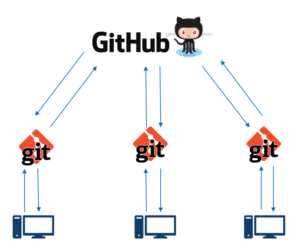
\includegraphics[width=0.5\textwidth]{GitHub-How-to-use-GitHub-Edureka-300x241.png}
%%  \url{https://www.edureka.co/blog/how-to-use-github/}
  \caption{GitHub is a cloud service that hosts code repositories which 
    you can access via a web browser.}
\end{figure}

\subsection{Objectives}
The assignment in this section is:
\begin{enumerate}
\item Create a GitHub account
\item Open the \code{src/hello.py} with GitHub Codespaces.
\item Run the \emph{tests}  in \code{tests/test\_hello.py}using Codespaces
\end{enumerate}

\subsection{Overview}

For this atelier you will use \textbf{GitHub CodeSpaces} as your
development environment.  This is a cloud-based interactive
development environment (IDE).  If you are interested in continuing to
work on the project after the atelier is finished today, you will
still be able to access GitHub CodeSpaces for as long as you wish in
the coming days, months, years.



You will start with existing code in a central repository of code, hosted by
GitHub on the cloud.  You will download (clone) a copy of this
repository, edit existing code, and create new code.

GitHub is a web based service which hosts thousands of projects, small
and large, in the cloud.  Typically, users have a development
environment on their local computer (laptop or desktop) and
periodically upload and download changes to the cloud.

The URL \url{https://github.com/jimka2001/immersion}, is the public
entry point to the GitHub project which we will work on in this
atelier.

You must create an account on GitHub (if you don't have one already).
This will be done in Section~\ref{sec.setup}.


\subsection{Getting Started}
\label{sec.setup}

We recommend you use the Chrome web browser.


\includegraphics[width=0.5\textwidth]{chrome.png}.

We need to set up the development environment.  The following steps should
help.

\subsection{Account Creation}
  
Create a GitHub account using an abstract user name.  Don't use your
real name.  Instead use an artificial name use as your name from
instagram or other social media.  You may also make up a completely
new name as long as no other person has already used that name on
GitHub.  \url{https://github.com/join}.  To complete the process of
creating a GitHub account you may need to authenticate using your
mobile phone.


\noindent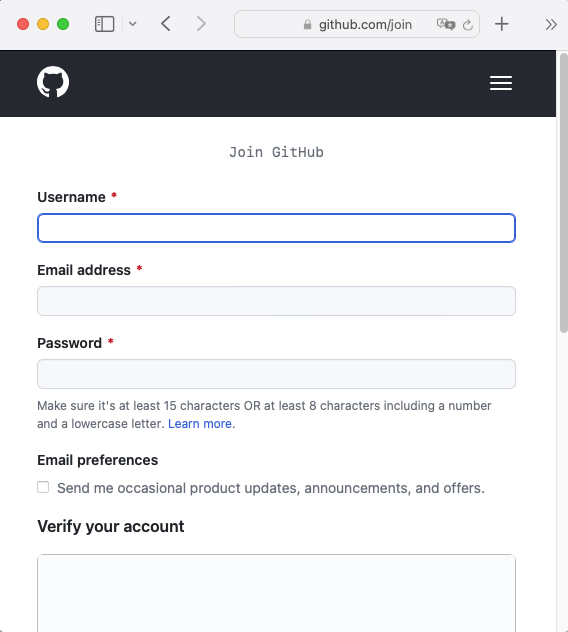
\includegraphics[width=0.5\textwidth]{github-join.png}



\subsection{Open the Repository}
  
Open \url{https://github.com/jimka2001/immersion} with your web browser.

\noindent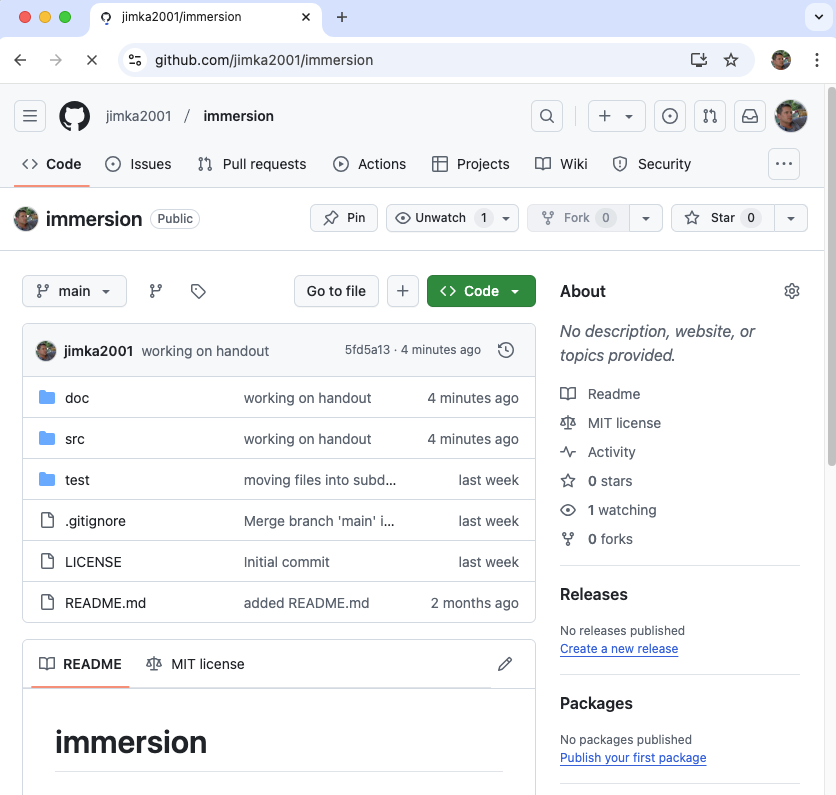
\includegraphics[width=0.5\textwidth]{github-immersion.png}


\subsection{Fork yourself a copy}

Fork the repository.  This gives you a private copy.  You will make changes
necessary changes in the code using this private copy.

\noindent 
\includegraphics[width=0.6\textwidth]{github-fork-repo.png}



\subsection{Open a Python File in Codespaces}
  
\begin{enumerate}
\item Navigate to \code{src/hello.py} to see something like this.

\noindent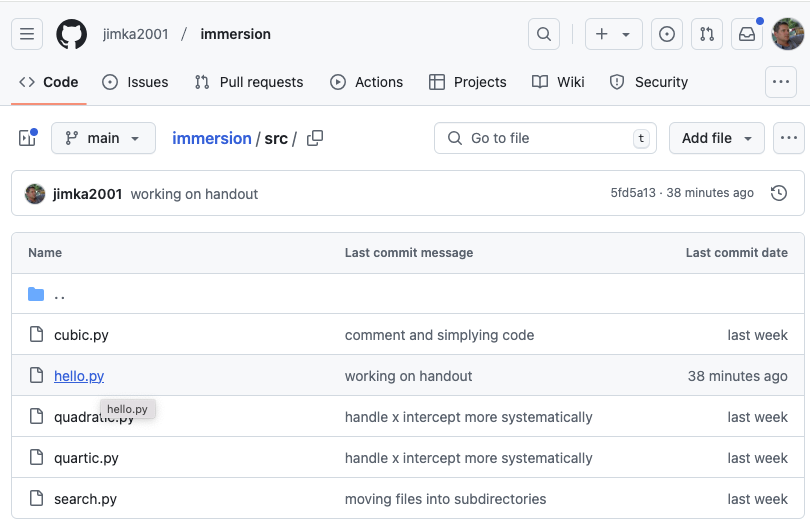
\includegraphics[width=0.9\textwidth]{find-hello.png}



\item Click \code{hello.py} to open the file in an editor pane.  You
  should see something like what is shown here:

\noindent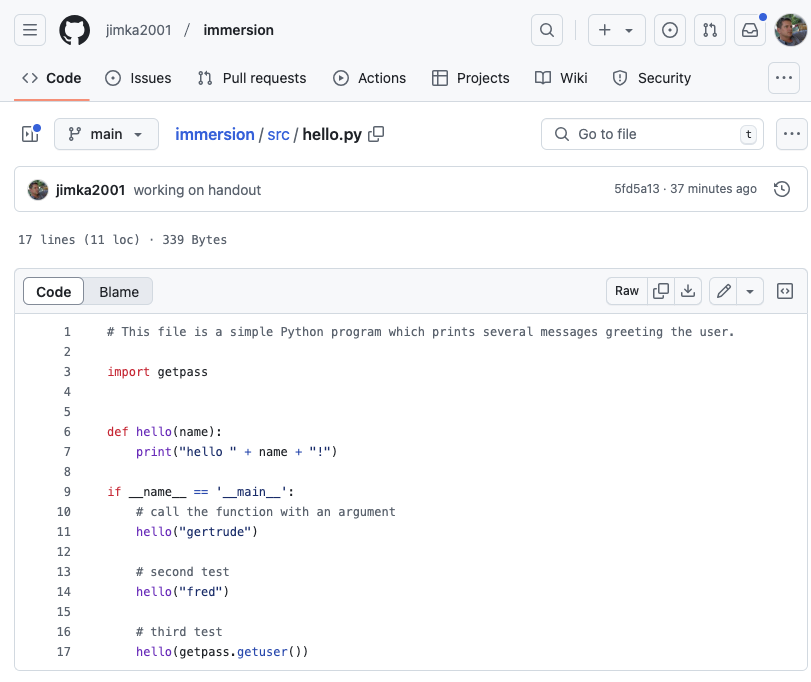
\includegraphics[width=0.9\textwidth]{hello-function.png}


\item Open the file by clicking \code{github.dev} not \code{Edit in place}.

\noindent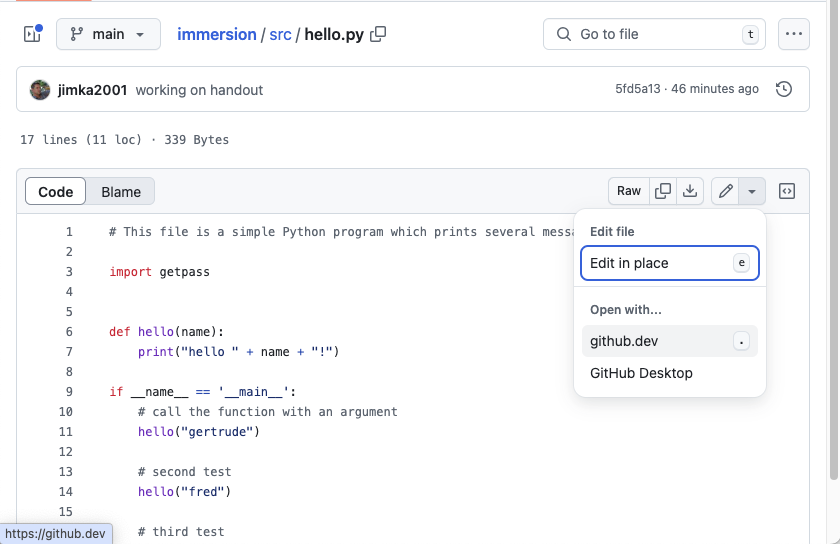
\includegraphics[width=0.9\textwidth]{github-dev.png}


\item You may need to wait while setting up. If this setup seems to
  never finish, it may mean you need to use Chrome as your web
  browser.

\noindent
\includegraphics[width=0.4\textwidth]{github-dev-setup.png}


\item GitHub may ask for permission to see your repository.  Click on \textbf{Allow}.
  
\noindent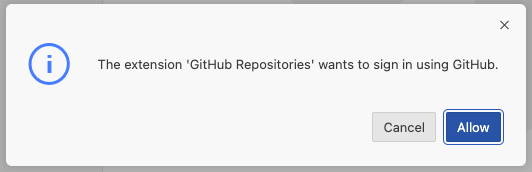
\includegraphics[width=0.7\textwidth]{github-ask-permission.png}
  

\item GitHub may ask for your GitHub ID.  Normally you just select the default one.
  
\noindent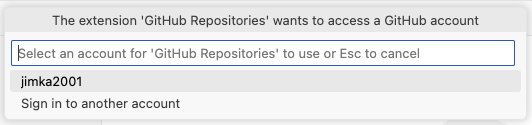
\includegraphics[width=0.5\textwidth]{github-ask-user-name.png}

\item Finally, the GitHub development environment should be opened.
  
\noindent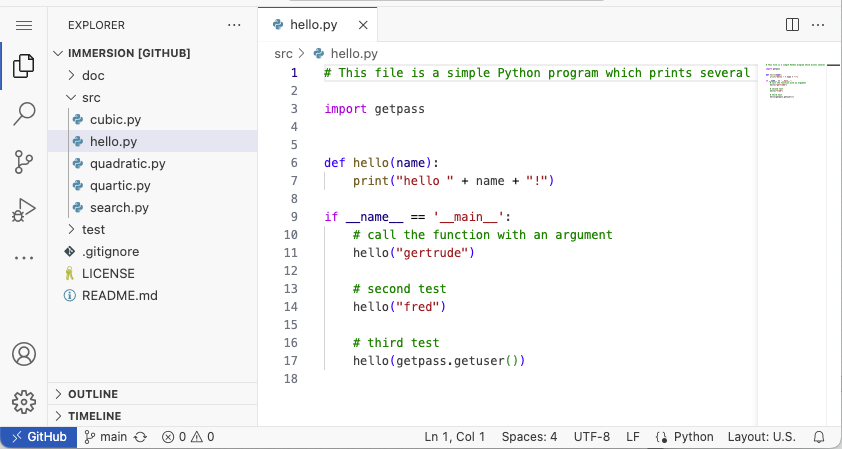
\includegraphics[width=0.6\textwidth]{github-dev-opened.png}



\end{enumerate}

\subsection{Set up the Editor}
  
\begin{enumerate}

\item Now you can edit your code but you cannot run nor test it.

\item Find the icon 
\includegraphics[width=2cm]{run-debug.png} on the left hand side of the browser window.   Press that icon to see the following message.

\noindent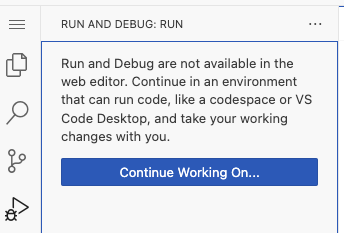
\includegraphics[width=0.6\textwidth]{continue.png}

\item Press continue, and you should see a prompt such as the following to create a code space.   

\noindent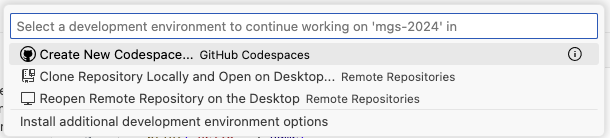
\includegraphics[width=0.9\textwidth]{create-code-space.png}

\item Select 
\includegraphics[width=8cm]{select-create.png}.

\item You may be asked how many cores do you want.

\noindent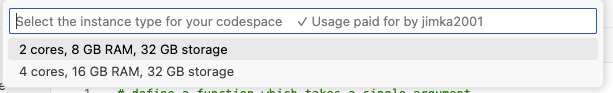
\includegraphics[width=0.9\textwidth]{select-cores.png}

\item You should select the minimum: 
\includegraphics[width=7cm]{two-cores.png}.

\item You'll probably now need to reopen the \code{src/hello.py} file.

\noindent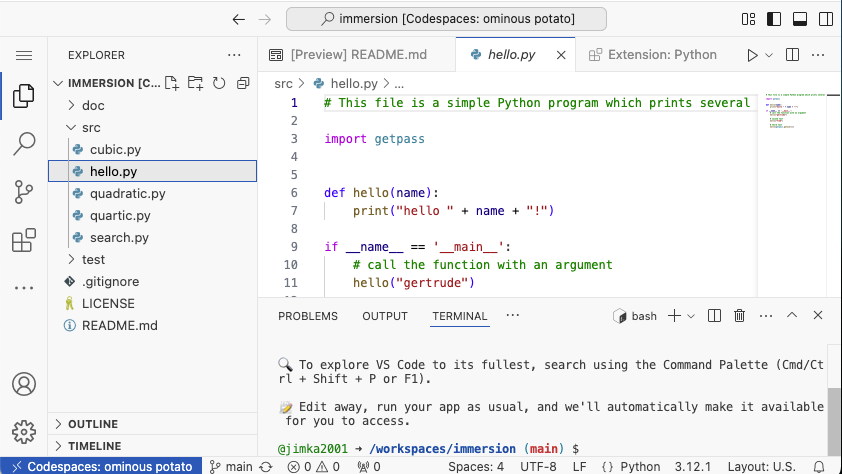
\includegraphics[width=0.9\textwidth]{re-open-python-file.png}

\item You may be asked to install the Python extension.  Press \textbf{Install}.

\noindent
\includegraphics[width=0.8\textwidth]{install-python-extension.png}

  

\item Wait until it finishes installing.  When it finishes installing, you should see something like this:

\noindent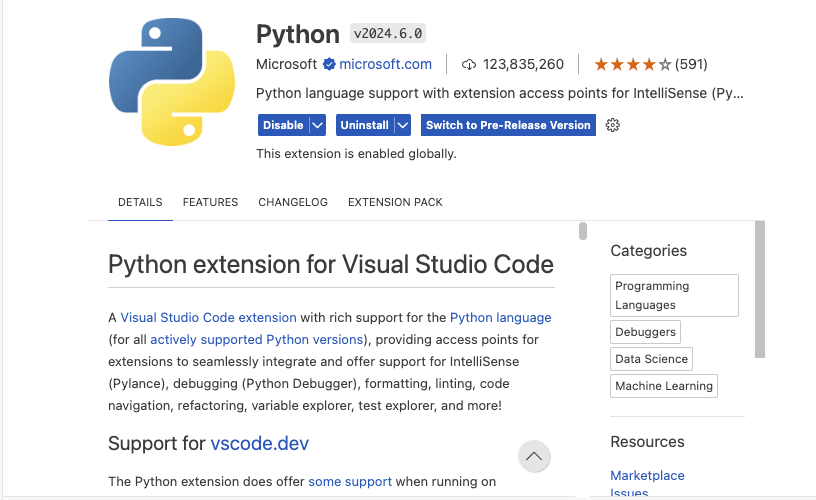
\includegraphics[width=0.9\textwidth]{python-extension.png}

\item Reopen the explorer: 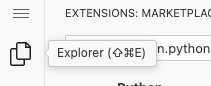
\includegraphics[width=7cm]{explorer2.png}, and select the \code{src/hello.py} file.

\noindent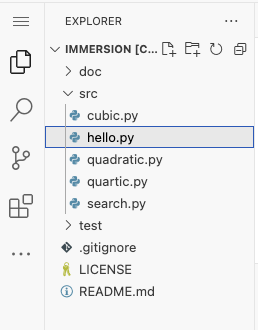
\includegraphics[width=0.4\textwidth]{explorer.png}
\end{enumerate}

\subsection{Example the Code}
Take a look at the Python code in the file \code{src/hello.py}.  In particular there are two sections in the code, 
\begin{enumerate}
\item A declaration of the function named \code{hello}, shown in Listing~\ref{list.hello}
\item Two conditional calls to the function \code{hello}, each time with a different argument, shown in Listing~\ref{list.calls}.
\end{enumerate}

\begin{listing}{Declaration of Function \code{hello}}{hello}
\begin{minipage}[c]{0.95\textwidth}\begin{lstlisting}
def hello(name):
    print("hello " + name + "!")
\end{lstlisting}\end{minipage}\end{listing}

\begin{listing}{Calls to Function \code{hello}}{calls}
\begin{minipage}[c]{0.95\textwidth}\begin{lstlisting}
if __name__ == '__main__':
    # call the function with an argument
    hello("gertrude")
    
    # second test
    hello("fred")
\end{lstlisting}\end{minipage}\end{listing}


\subsection{Make a Sample Run}

Find the icon 
\includegraphics[height=1.0cm]{run-triangle.png}
  in the top-right of the editor window.  Click the triangle, to see a sample run/execution of the code.

\noindent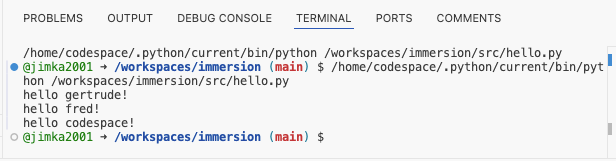
\includegraphics[width=\textwidth]{hello-terminal-output.png}


\subsection{Running Predefined Tests}
\label{sec.run.tests}

Open the file \code{tests/test\_hello.py} in a GitHub Codespace.

\noindent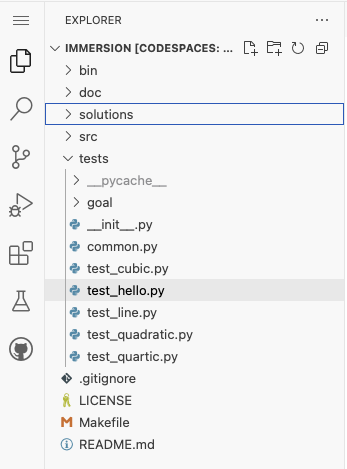
\includegraphics[width=0.4\textwidth]{test-hello-explorer.png}

To run the tests, press the 
\includegraphics[width=1cm]{run-triangle.png} which
you should find in the upper-right corner of the editor window.

\noindent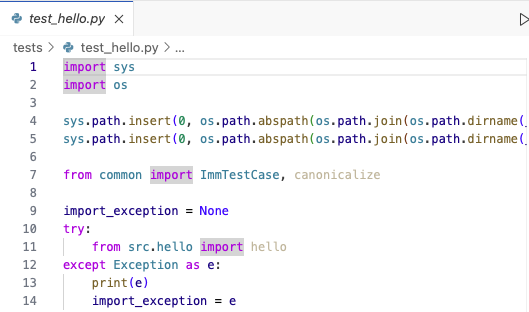
\includegraphics[width=0.8\textwidth]{hello-test.png}



\subsection{Challenges for the Student}

Understanding errors and debugging is difficult, but it is part of programming.

Experiment with the simple pieces of code in the above sections.
Insert spaces and press the run button.  Look at the error messages
produced. Remove some quotation marks or parentheses (leaving
unbalanced quotations marks or parentheses)---again look at what error
messages you see when you try to run invalid code.


\begin{enumerate}
\item Remove and add some spaces at the beginning of a line.
\item Change the indentation.
\item Unbalance the parentheses.
\item Unbalance the quotation marks.
\item Put extra spaces inside the quotation marks.
\item Change the name of the \code{hello} function at definition site or call site.
\item Figure out how to undo your changes in the editor to make the code work again.
\item Run the tests \code{test/test\_hello.py} as explained in Section~\ref{sec.run.tests}.
\end{enumerate}

\clearpage

\pagebreak
\section{Hello World}
\label{sec.hello.world}

The first program we usually write in any programming language is
called \code{hello-world}.  It is a very simple program.  However
getting it to run means you have to understand how to use the
programming environment.

\subsection{Examine the Code}
\label{sec.examine.the.code}
Take a look at the Python code in the file \code{src/hello.py}.  In
particular there are two sections in the code,
\begin{enumerate}
\item A declaration of the function named \code{hello}, shown in
  Listing~\ref{list.hello}
\item Two conditional calls to the function \code{hello}, each time
  with a different argument, shown in Listing~\ref{list.calls}.
\end{enumerate}

\begin{listing}{Declaration of Function \code{hello}}{hello}
\begin{minipage}[c]{0.95\textwidth}\begin{lstlisting}
def hello(name):
    print("hello " + name + "!")
\end{lstlisting}\end{minipage}\end{listing}

\begin{listing}{Calls to Function \code{hello}}{calls}
\begin{minipage}[c]{0.95\textwidth}\begin{lstlisting}
if __name__ == '__main__':
    # call the function with an argument
    hello("gertrude")
    
    # second test
    hello("fred")
\end{lstlisting}\end{minipage}\end{listing}


\subsection{Make a Sample Run}

Find the icon 
\includegraphics[height=1.0cm]{run-triangle.png} in the
top-right of the editor window.  Click the triangle, to see a sample
run/execution of the code.

\noindent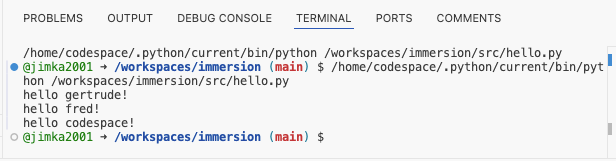
\includegraphics[width=\textwidth]{hello-terminal-output.png}


\subsection{Running Predefined Tests}
\label{sec.run.tests}

Open the file \code{tests/test\_hello.py} in a GitHub Code-Space.

\noindent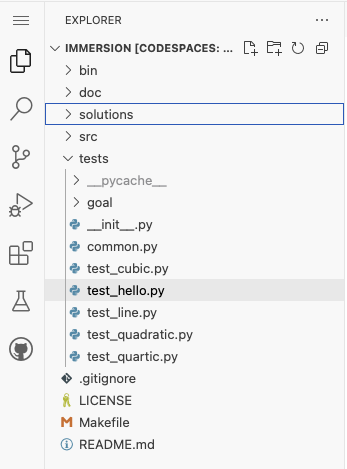
\includegraphics[width=0.4\textwidth]{test-hello-explorer.png}

To run the tests, press the

\includegraphics[width=1cm]{run-triangle.png} which you should find in
the upper-right corner of the editor window.

\noindent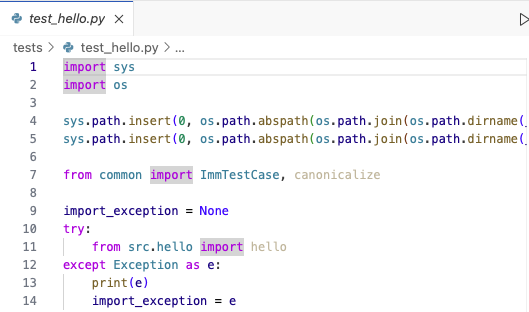
\includegraphics[width=0.8\textwidth]{hello-test.png}


The text window at the bottom of the editor should show the results of
how many tests ran and whether there are any failures.

\noindent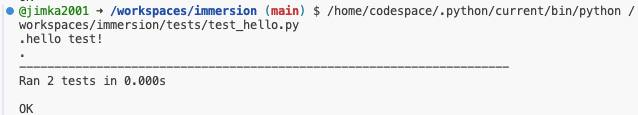
\includegraphics[width=0.9\textwidth]{github-test-result.png}



\subsection{Challenges for the Student}

Understanding errors and debugging is difficult, but it is part of
programming.

Experiment with the simple pieces of code in the above sections.
Insert spaces and press the run button.  Look at the error messages
produced. Remove some quotation marks or parentheses (leaving
unbalanced quotations marks or parentheses)---again look at what error
messages you see when you try to run invalid code.


\begin{enumerate}
\item Remove and add some spaces at the beginning of a line.
\item Change the indentation.
\item Unbalance the parentheses.
\item Unbalance the quotation marks.
\item Put extra spaces inside the quotation marks.
\item Change the name of the \code{hello} function at definition site
  or call site.
\item Figure out how to undo your changes in the editor to make the
  code work again.
\item Run the tests \code{test/test\_hello.py} as explained in
  Section~\ref{sec.run.tests}.
\end{enumerate}

\clearpage

% LocalWords:  GitHub png github
\pagebreak\mbox{}\pagebreak
\setcounter{page}{0}
%\thispagestyle{empty}
\section{Review of Polynomials (Optional)}
\label{sec.general}

Your goal in the next several sections is to find \emph{root} of \emph{polynomials}
But first, what is a polynomial? And then, what is a root?

\begin{definition}{polynomial of degree n}{}
  A \emph{polynomial} of \emph{degree n} is a function of a single variable, usually $x$,
  of the form.
  \[P(x) = \alpha_n x^n + \alpha_{n-1} x^{n-1} + \cdots + \alpha_2 x^2 + \alpha_1 x + \alpha_0 \]

  where $\alpha_n,  \alpha_{n-1} x^{n-1}, \ldots, \alpha_0$ are called coefficients and may be integers, rational numbers, or real numbers.
\end{definition}

An example of a 4th degree polynomial is
\[P(x) = 2 x^4 + 5 x^3 + x^2 - x + 1\,.\]


Any of the coefficients after the leading one may be 0, in which case the term is generally omitted.
An example of a 3th degree polynomial where the coefficients of the $x^2$ term is 0 is as follows.
\[P(x) = 5 x^3 + x - 1\,.\]

\begin{definition}{root}{}
  If $P(x)$ is a polynomial, and $r$ is a number for which $P(r)=0$, then $r$ is called a \emph{root}
  of the polynomial.
\end{definition}

The polynomial $P(x) = x^3 - x$ as three roots, 1, -1, and 0.  We know this because
\begin{align*}
  P(1) &= (1)^3 - 1 
  = 1 - 1 
  = 0\\[3pt]
  P(-1) &= (-1)^3 - (-1) 
  = -1 + 1 
  = 0\\[3pt]
  P(0) &= (0)^3 - 0
  = 0 - 0 
  = 0  
\end{align*}

\begin{theorem}{Fundamental Theorem of Algebra}{ftoa}
  Every non-constant polynomial of degree 1 or higher has a root.
\end{theorem}

The Fundamental Theorem of Algebra claims that every polynomial.  However, sometimes the root is complex.
For example the polynomial, $P(x) = x^2 + 1$, has two comples roots.
In this atelier, we we only attempt to determine the real roots, ignoring the complex roots.
For this reason, we will not be able to find all the roots of some polynomials.

\begin{corollary}{Roots with Multiplicity}{n.roots}
  A polynomial of degree $n\ge 1$ has $n$ roots, some of which may be equal.
\end{corollary}
\begin{proof}

  [By Induction]
  
  \begin{itemize}
    
  \item \textbf{Base case:} If $n=1$, then Theorem~\ref{th.ftoa}
    guarantees it has a root; call it $r_1$.  Thus it is of the form
    $P(x)=\alpha (x-r_1)$.
  \item \textbf{Inductive case:} Suppose $n>1$.  Suppose every polynomial, $Q(x)$ of degree
    $n$ has $n$-many roots, $r_1,\ldots,r_n$, and can thus be written as:
    \[Q(x) = \alpha_1 (x - r_1) (x - r_2) \cdots (x - r_n)\]
    Now consider a polynomial, $P(x)$, of
    degree $n+1$.  Theorem~\ref{th.ftoa} guarantees $P(x)$ has a root;
    call it $r_{n+1}$, thus $(x-r_{n+1})$ is a factor of $P(x)$ so there
    exists a polynomial, $Q(x)=$, of degree $n$ such that
    $P(x) =  Q(x) (x-r_{n_1})$.
    But by inductive hypothesis, $Q(x)$ can be written
    as \[Q(x) = \alpha_1 (x - r_1) (x - r_2) \cdots (x - r_n)\]
    So, \[P(x) = \alpha_1 (x - r_1) (x - r_2) \cdots (x - r_n) (x-r_{n+1})\]

    Thus $P(x)$ has $n+1$ roots.
  \end{itemize}
\end{proof}

Corollary~\ref{cor.n.roots} can be seen as a model of how we will find
roots in this attempt.  Given a degree $n$ polynomial (for $2<n\leq
5$), if we successfully find a root, $r_n$, then we will factor
$(x-r_n)$ out of the polynomial, giving us new polynomial but with
degree $n-1$, which we can solve by the same approach.  This process
continues until we reach degree $n=2$ which we solve using the
quadratic formula.
\pagebreak
\section{The Line: degree=1}
\label{sec.line}

\begin{figure}
  \centering
  %% derived from https://tex.stackexchange.com/questions/357538/graph-of-a-parabola-on-pgfplots
%% Thanks to Stefan Pinnow
%%     https://tex.stackexchange.com/users/95441/stefan-pinnow

\begin{figure}
\centering
\begin{tikzpicture}
    \begin{axis}[
        width=3in,
        height=3in,
        axis lines=middle,
        xmin=-10,
        xmax=10,
        ymin=-10,
        ymax=10,
%        xtick={1,1},
        % ---------------------------------------------------------------------
        % you don't want the ticks/tick labels to be scaled
        scaled ticks=false,
%        % and the tick labels are shown by default the way you want them,
%        % so you don't need to specify them explicitely
%        xticklabels={$20000$},
        % ---------------------------------------------------------------------
%        ytick={\empty},
        ticklabel style={font=\scriptsize},
        xlabel=$x$,
        ylabel=$y$,
        axis line style={
            latex-latex,
            shorten >=-12.5pt,
            shorten <=-12.5pt,
        },
        xlabel style={at={(ticklabel* cs:1)}, xshift=12.5pt, anchor=north west},
        ylabel style={at={(ticklabel* cs:1)}, yshift=12.5pt, anchor=south west},
    ]

        \addplot[samples=51,smooth,domain=-10:10] {-1.2*x + 3};
    \end{axis}

\end{tikzpicture}

\caption{Line: $y = P(x) = -1.2*x + 3$}
\label{fig.line}
\end{figure}

  \caption{Line: $y = P(x) = -1.2*x + 3$}
  \label{fig.line}
\end{figure}


\subsection{Objectives}
The assignment in this section is:
\begin{enumerate}
\item Complete the file \code{src/line.py} by writing a Python
  function which computes and returns the x-intercept of a line whose
  equation is ${y=a x + b}$.
\item You'll need to replace all occurrences of \code{raise
  NotImplementedError()} with correct python code which passes the
  tests.

\item Test the function in GitHub Code-Spaces by running the file\\
  \code{test/test\_line.py}.
\end{enumerate}

\subsection{Overview}


A polynomial of degree~1 is a function $P(x)=a x + b$ whose graph is a
line.  If $a=0$ the line is horizontal an crosses the y-axis at $y=b$;
thus if $b\neq 0$ then $P(x)\neq 0$.  So if $a=0$ we will assume that
$P(x)$ has no root.

\subsection{The Math / The Theoretical}


Figure~\ref{fig.line} shows the graphs of two polynomials of degree~1.

\begin{align*}
  P_1(x) &= -1.2 x + 3\\
  P_2(x) &= 0 x + 6
\end{align*}

The line representing $P_1(x)$ has an x-intercept computed as in
Example~\ref{ex.line}.


\begin{example}{Computing x-intercept of a line}{line}
  \begin{align*}
  P_1(x) &= a x + b \\
  0  &= -1.2 x + 3\\
  x &= \frac{3}{1.2} = 2.5
  \end{align*}
\end{example}

We see in Figure~\ref{fig.line} that if the coefficient of $x$ is 0,
then the line is horizontal and has no x-intercept. $P_2(x)$ is an
example where $a=0$.  If the horizontal line $P_2(x)$is coincident
with the x-axis, \ie, if $a=0$ and $b=0$, then there is no unique
x-intercept.





If $a\neq 0$, then we have a line as shown in Figure~\ref{fig.line}.
We can solve for the x-intercept by setting y to 0 and solving for x.
\begin{align*}
  y &= a x + b\\
  0 &= a x + b\\
  -b &= a x\\
  \frac{-b}{a} &= x
\end{align*}



\subsection{The Programming / The Practical}


\begin{listing}{Function declaration to find x-intercept of a line.}{code.line}
\begin{minipage}[c]{0.95\textwidth}\begin{lstlisting}
def find_x_intercept(a,b):
    if a == 0:
        # CHALLENGE: student must complete the implementation.
        raise NotImplementedError()

    else:
        # CHALLENGE: student must complete the implementation.
        raise NotImplementedError()
\end{lstlisting}\end{minipage}\end{listing}


\begin{enumerate}

\item Open the file \code{src/line.py} in your web-based editor
  (GitHub Code-Spaces).  You will develop the code in this file.

\item Find the occurrences of \code{raise NotImplementedError()}.
  This is the code that you must replace with working Python code.

\item You should update the code in the file \code{src/line.py} so
  that if $a$ is 0, then the function returns an empty list and
  otherwise returns a list of the value~$\frac{-b}{a}$.

\item You must figure out how to write that in the Python language.
  \Ie, you must figure out how to divide two numbers in Python and how
  to create a list, empty and otherwise.


\item Test your code by running the pre-defined tests in \\
  \code{tests/test\_line.py}.

\item Look at the proposed solution in \code{solutions/line.py}.  It
  is not necessary that your code match exactly.

\end{enumerate}

% LocalWords:  GitHub NotImplementedError
\pagebreak
\section{Quadratic: degree=2}
\label{sec.quadratic}

%% derived from https://tex.stackexchange.com/questions/357538/graph-of-a-parabola-on-pgfplots
%% Thanks to Stefan Pinnow
%%     https://tex.stackexchange.com/users/95441/stefan-pinnow

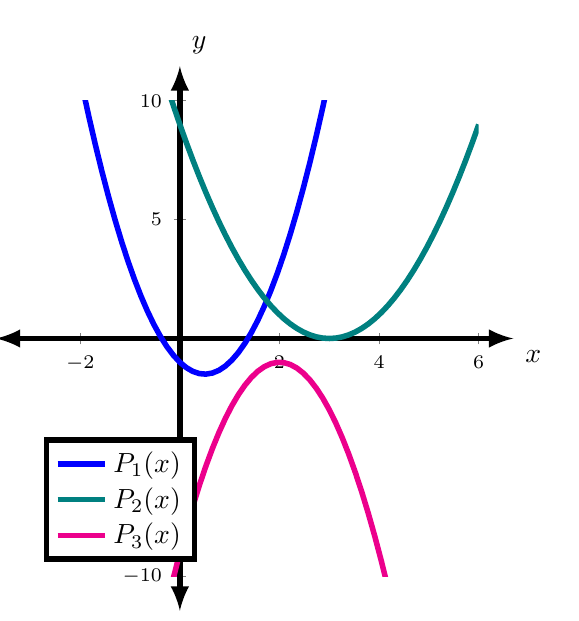
\begin{tikzpicture}
  \begin{axis}[
      legend pos=south west,
      width=.6\textwidth,
      height=3in,
      axis lines=middle,
      xmin=-3,
      xmax=6,
      ymin=-10,
      ymax=10,
      scaled ticks=false,
      line width=2pt,
      ticklabel style={font=\scriptsize},
      xlabel=$x$,
      ylabel=$y$,
      samples=70,
      domain=-3:6,
      axis line style={
        latex-latex,
        shorten >=-12.5pt,
        shorten <=-12.5pt,
      },
      xlabel style={at={(ticklabel* cs:1)}, xshift=12.5pt, anchor=north west},
      ylabel style={at={(ticklabel* cs:1)}, yshift=12.5pt, anchor=south west},
    ]
    
    \addplot[color=blue] {2*x^2 - 2*x - 1}; % 2 roots
    \addlegendentry{\(P_1(x)\)}
    \addplot[color=teal] {x^2 - 6*x + 9}; % 1 root
    \addlegendentry{\(P_2(x)\)}
    \addplot[color=magenta] {-2*x^2 + 8*x - 9}; % 0 roots
    \addlegendentry{\(P_3(x)\)}
  \end{axis}
\end{tikzpicture}
%


A quadratic polynomial is of the form $P(x)=a x^2 + b x + c$.  If
$a=0$, then $P(x)$ is actually a first degree polynomial which can be
solved using the techniques described in Section~\ref{sec.line}.

We have the plots of three quadratic polynomials, $P_1(x)$, $P_2(x)$,
and $P_3(x)$, shown in Figure~\ref{fig.parabola}.  Each plot takes the
geometric form of a parabola.  As can be seen in the figure, the
parabola might intersect the x-axis twice (\eg, $P_1(x)$), once (\eg,
$P_2(x)$, or not at all (\eg, $P_3(x)$).

\begin{align*}
  P_1(x) &= 2x^2 - 2 x - 5\\
  P_2(x) &= x^2 -x + \frac{1}{4}\\
  P_3(x) &=  -2x^2 + 2x -2
\end{align*}


\subsection{Mathematically Computing the Roots of a Quadratic}

To determine how many times a parabola touches the x-axis, we need to
find the roots of the corresponding quadratic (degree 2) polynomial of
the form $a x^2 + b x + c$.  The formula is called the \emph{quadratic
formula} is given in Equation~\eqref{eq.quad.formula}.  In particular,
we need to look at the expression under the square root, called the
discriminant: $b^2 - 4a c$.
\begin{itemize}
\item If the discriminant is positive, then the polynomial has two
  distinct real roots.
\item If the discriminant is zero, then the positive and negative
  square roots are both 0; thus the polynomial has 1 single root.
\item If the discriminant is negative, then there is a negative under
  the radical sign; thus the polynomial has no real roots.  The
  polynomial does have complex roots; however we will ignore complex
  roots for this atelier.
\end{itemize}

Example~\ref{ex.degree2.p1} shows the computation of the two distinct roots of $P_1(x)$.

\begin{example}{Explicit Computation of Roots of $P_1(x)$}{degree2.p1}
  $P_1(x)$, has two roots.  They can be found using the quadratic formula.
  \begin{align*}
    a&=2\\
    b&=-2\\
    c&=-5\\
    b^2 - 4a c &= (-2)^2 - 4 (2) (-5)\\
    &= 4 + 40 = 44\\
    \sqrt{b^2 - 4a c} &= \sqrt{44} = 2\sqrt{11}
  \end{align*}

\begin{align}
  x &= \frac{-b~ \pm \sqrt{b^2 - 4a c}}{2a}\label{eq.quad.formula}\\
  &= \frac{-(-2)~ \pm 2\sqrt{11}}{(2)(2)}\nonumber\\
  &= \frac{2 ~\pm 2\sqrt{11}}{4}
  = \frac{1}{2} \pm \frac{1}{2}\sqrt{11}\nonumber
\end{align}
  
\end{example}

Example~\ref{ex.degree2.p2} shows the computation of the root of $P_2(x)$.

\begin{example}{Explicit Computation of Root of $P_2(x)$}{degree2.p2}
In the case of $P_2(x) = x^2 -x + \frac{1}{4}$, we do a similar computation.

\begin{align*}
  a &= 1\\
  b &= -1\\
  c &= \frac{1}{4} \\
  b^2 - 4a c &= (-1)^2 - 4 (1) (\frac{1}{4})\\
  &= 1 - 1 = 0
\end{align*}

\begin{align*}
  x &= \frac{-b~ \pm \sqrt{b^2 - 4a c}}{2a}\\
  &= \frac{-(-1)~ \pm \sqrt{0}}{(2)(1)}\\
  &= \frac{1}{2}
\end{align*}


Thus there is exactly one root.  The existance of the single root can be
seen in Figure~\ref{fig.parabola} by the fact that the
parobala touches the x-axis tangentially.
\end{example}

Example~\ref{ex.degree2.p3} examines $P_3(x)$.

\begin{example}{Examination of $P_3(x)$}{degree2.p3}
  In the case of $P_3(x) = -2x^2 + 2x -2$, we may attempt the same but we have a negative discriminant.
  \begin{align*}
    a&=-2\\
    b&=2\\
    c&=-2\\
    b^2 - 4a c  &=(-2)^2 - (4)(-2)(-2)\\
    &= 4 - 16 = -12 < 0
  \end{align*}

When the discriminant
is negative, there are no \emph{real} roots.  This can be seen in
Figure~\ref{fig.parabola} by the fact that the parobola does not
touch the x-axis at all.
\end{example}

\subsection{Programmatically Computing Roots of a Quadratic}

Steps for computing roots of a polynomial of degree 2.
\begin{enumerate}
\item Assume the coefficients of $P(x)$ are in the variables \code{a}, \code{b}, and \code{c}.
\item If \code{a == 0}, then delegate to previous solution by calling the function \code{find\_x\_intercept} and returning its value.  Note that \\
  \code{find\_x\_intercept} takes two arguments, which it calls \code{a} and \code{b}, but these are not \code{a} and \code{b} of the quadratic.   In fact for \code{find\_x\_intercept}, \code{a} is the coefficients of $x$ and \code{b} is the bias term of $a x + b$.  However, for the quadratic, \code{a} is the coefficient of $x^2$, and \code{b} is the code of $x$ in $a x^2 + b x + c$.
\item Compute the discriminant, storing in the variable \code{discriminant}.
\item Test three conditions.
  \begin{enumerate}
  \item If the discriminant is positive, then return a list of the two roots.
  \item If the discriminant is zero (or very close to zero), then return a list (of length two) of the same root twice.
  \item If the discriminant is negative ( $< -\varepsilon$), then return an empty list~\code{[]}.
  \end{enumerate}
\end{enumerate}


\begin{listing}{Function to compute roots of a quadratic polynomial.}{code.quadratic}
\begin{minipage}[c]{0.95\textwidth}\begin{lstlisting}
def find_quadratic_roots(a, b, c):
    epsilon = 0.001
    discriminant = b * b - 4 * a * c
    if a == 0:
        # CHALLENGE: student must complete the implementation.
        raise NotImplementedError()

    if abs(discriminant) < epsilon:
        # CHALLENGE: student must complete the implementation.
        raise NotImplementedError()

    elif discriminant > 0:
        # CHALLENGE: student must complete the implementation.
        raise NotImplementedError()

    else:
        # CHALLENGE: student must complete the implementation.
        raise NotImplementedError()

\end{lstlisting}\end{minipage}\end{listing}

\pagebreak
\section{Cubic: degree=3}
\label{sec.cubic}

We have a two cubic equations plotted in Figure~\ref{fig.cubic}.
%% derived from https://tex.stackexchange.com/questions/357538/graph-of-a-parabola-on-pgfplots
%% Thanks to Stefan Pinnow
%%     https://tex.stackexchange.com/users/95441/stefan-pinnow

\begin{figure}
\centering
\begin{tikzpicture}
    \begin{axis}[
        width=3in,
        height=3in,
        axis lines=middle,
        xmin=-5,
        xmax=6,
        ymin=-50,
        ymax=60,
%        xtick={20000},
        % ---------------------------------------------------------------------
        % you don't want the ticks/tick labels to be scaled
        scaled ticks=false,
%        % and the tick labels are shown by default the way you want them,
%        % so you don't need to specify them explicitely
%        xticklabels={$20000$},
        % ---------------------------------------------------------------------
 %       ytick={\empty},
        ticklabel style={font=\scriptsize},
        xlabel=$x$,
        ylabel=$y$,
        axis line style={
            latex-latex,
            shorten >=-12.5pt,
            shorten <=-12.5pt,
        },
        xlabel style={at={(ticklabel* cs:1)}, xshift=12.5pt, anchor=north west},
        ylabel style={at={(ticklabel* cs:1)}, yshift=12.5pt, anchor=south west},
    ]

        \addplot[samples=51,smooth,domain=-10:10] {x^3 - 4*x^2 - 2*x - 10};

    \end{axis}


\end{tikzpicture}
\caption{Cubic: $y=P(x) = x^3 - 4*x^2 - 2*x - 10$}
\label{fig.cubic}
\end{figure}

\begin{align*}
  P_1(x) &= x^3 - 4*x^2 - 2*x - 10\\
  P_2(x) = -P_1(x) &= -x^3 + 4*x^2 + 2*x + 10
\end{align*}


\begin{listing}{Function to compute roots of cubic polynomial.}{code.cubic}
\begin{minipage}[c]{0.98\textwidth}\begin{lstlisting}
def find_cubic_roots(a, b, c, d):
    epsilon = 0.00001
    if a == 0:
        return find_quadratic_roots(b, c, d)
    if a < 0:
        return find_cubic_roots(-a, -b, -c, -d)

    f = make_cubic(a, b, c, d)

    # f(0) = d
    if d == 0.0:
        r = 0.0
    elif d > 0: # f(0) > d, so f(-infinity) < 0 and f(infinity) > 0
        r = search_root_left(-1, 0, f, epsilon)
    else:
        r = search_root_right(0, 1, f, epsilon)
    return factor_out_cubic_root(r, a, b, c)
\end{lstlisting}\end{minipage}\end{listing}
\pagebreak
\section{Quartic}
\label{sec.quartic}



\lipsum[9-10] %% replace this line with your text


We have two quartic equations plotted in Figure~\ref{fig.quartic}.
%% derived from https://tex.stackexchange.com/questions/357538/graph-of-a-parabola-on-pgfplots
%% Thanks to Stefan Pinnow
%%     https://tex.stackexchange.com/users/95441/stefan-pinnow

\begin{figure}
\centering
\begin{tikzpicture}
    \begin{axis}[
        width=3in,
        height=3in,
        axis lines=middle,
        xmin=-5,
        xmax=12,
        ymin=-60,
        ymax=60,
%        xtick={20000},
        % ---------------------------------------------------------------------
        % you don't want the ticks/tick labels to be scaled
        scaled ticks=false,
%        % and the tick labels are shown by default the way you want them,
%        % so you don't need to specify them explicitely
%        xticklabels={$20000$},
        % ---------------------------------------------------------------------
 %       ytick={\empty},
        ticklabel style={font=\scriptsize},
        xlabel=$x$,
        ylabel=$y$,
        axis line style={
            latex-latex,
            shorten >=-12.5pt,
            shorten <=-12.5pt,
        },
        xlabel style={at={(ticklabel* cs:1)}, xshift=12.5pt, anchor=north west},
        ylabel style={at={(ticklabel* cs:1)}, yshift=12.5pt, anchor=south west},
    ]

        \addplot[samples=51,smooth,domain=-4:12,color=blue] {0.125 * x^4 -2* x^3 + 7 * x^2 + x + 6};

    \end{axis}


\end{tikzpicture}
%
\begin{tikzpicture}
    \begin{axis}[
        width=3in,
        height=3in,
        axis lines=middle,
        xmin=-5,
        xmax=12,
        ymin=-60,
        ymax=60,
%        xtick={20000},
        % ---------------------------------------------------------------------
        % you don't want the ticks/tick labels to be scaled
        scaled ticks=false,
%        % and the tick labels are shown by default the way you want them,
%        % so you don't need to specify them explicitely
%        xticklabels={$20000$},
        % ---------------------------------------------------------------------
 %       ytick={\empty},
        ticklabel style={font=\scriptsize},
        xlabel=$x$,
        ylabel=$y$,
        axis line style={
            latex-latex,
            shorten >=-12.5pt,
            shorten <=-12.5pt,
        },
        xlabel style={at={(ticklabel* cs:1)}, xshift=12.5pt, anchor=north west},
        ylabel style={at={(ticklabel* cs:1)}, yshift=12.5pt, anchor=south west},
    ]

        \addplot[samples=51,smooth,domain=-4:12,color=blue] {-0.125 * x^4 +2* x^3 - 7 * x^2 - x - 6};

    \end{axis}


\end{tikzpicture}
\caption{Quartics: [left] ${y=P_1(x) = \frac{1}{8}  x^4 -2 x^3 + 7  x^2 + x + 6}$ \\[2pt]
[right] ${y=P_2(x) = -P_1(x) = -\frac{1}{8}  x^4 +2 x^3 - 7  x^2 - x - 6}$}
\label{fig.quartic}
\end{figure}


%% derived from https://tex.stackexchange.com/questions/357538/graph-of-a-parabola-on-pgfplots
%% Thanks to Stefan Pinnow
%%     https://tex.stackexchange.com/users/95441/stefan-pinnow

\begin{figure}
\centering
\begin{tikzpicture}
    \begin{axis}[
        width=3in,
        height=3in,
        axis lines=middle,
        xmin=-5,
        xmax=12,
        ymin=-60,
        ymax=60,
%        xtick={20000},
        % ---------------------------------------------------------------------
        % you don't want the ticks/tick labels to be scaled
        scaled ticks=false,
%        % and the tick labels are shown by default the way you want them,
%        % so you don't need to specify them explicitely
%        xticklabels={$20000$},
        % ---------------------------------------------------------------------
 %       ytick={\empty},
        legend pos=south west,
        ticklabel style={font=\scriptsize},
        xlabel=$x$,
        ylabel=$y$,
        axis line style={
            latex-latex,
            shorten >=-12.5pt,
            shorten <=-12.5pt,
        },
        xlabel style={at={(ticklabel* cs:1)}, xshift=12.5pt, anchor=north west},
        ylabel style={at={(ticklabel* cs:1)}, yshift=12.5pt, anchor=south west},
    ]


    \end{axis}


\end{tikzpicture}
%
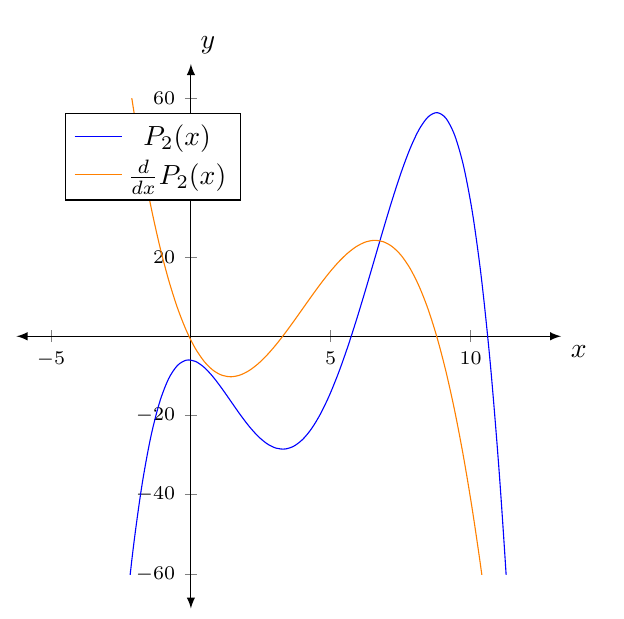
\begin{tikzpicture}
  \begin{axis}[
      width=3in,
      height=3in,
      axis lines=middle,
      xmin=-5,
      xmax=12,
      ymin=-60,
      ymax=60,
      scaled ticks=false,
      legend pos=north west,
      ticklabel style={font=\scriptsize},
      xlabel=$x$,
      ylabel=$y$,
      axis line style={
        latex-latex,
        shorten >=-12.5pt,
        shorten <=-12.5pt,
      },
      xlabel style={at={(ticklabel* cs:1)}, xshift=12.5pt, anchor=north west},
      ylabel style={at={(ticklabel* cs:1)}, yshift=12.5pt, anchor=south west},
    ]
    
    \addplot[samples=51,smooth,domain=-4:12,color=blue] {-0.125 * x^4 +2* x^3 - 7 * x^2 - x - 6};
    \addlegendentry{\(P_2(x)\)}
    \addplot[samples=51,smooth,domain=-4:12,color=orange] {-0.5 * x^3 +6* x^2 - 14 * x - 1};
    \addlegendentry{\(\frac{d}{dx}P_2(x)\)}
  \end{axis}
\end{tikzpicture}
\caption{Quartics $P_1(x)$ and $P_2(x)$ from Figure~\ref{fig.quartic} and their derivatives.
  \textcolor{blue}{In blue ${y=P_1(x)}$ and ${y=P_2(x)}$}.
  \textcolor{orange}{In orange ${y=-\frac{d}{dx} P_1(x)}$ and ${y=-\frac{d}{dx} P_2(x)}$}}
\label{fig.quartic.deriv}
\end{figure}

\pagebreak
\section{Quintic: degree=5}
\label{sec.quintic}

This exercise is left as an exercise for the student.  However, the following are some
notes to help lead the student in the right direction.

\begin{figure}
\centering
%% derived from https://tex.stackexchange.com/questions/357538/graph-of-a-parabola-on-pgfplots
%% Thanks to Stefan Pinnow
%%     https://tex.stackexchange.com/users/95441/stefan-pinnow

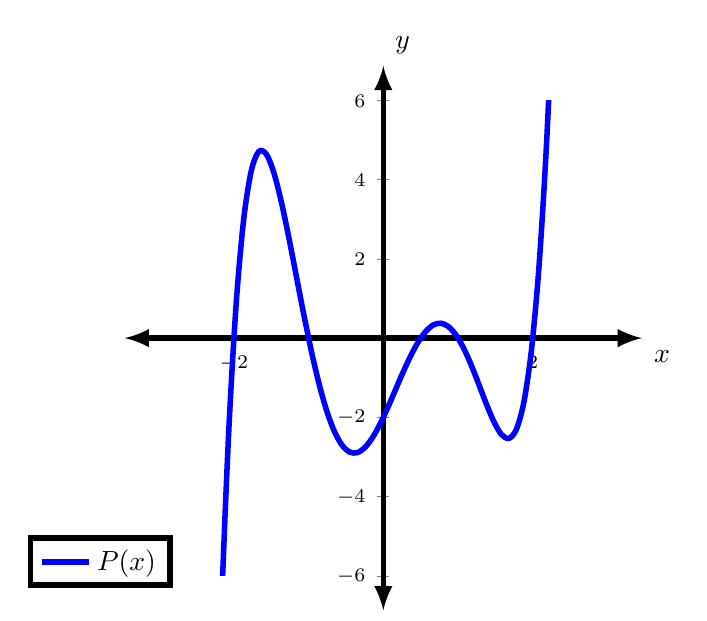
\begin{tikzpicture}
  \begin{axis}[
      samples=70,
      smooth,
      line width=2pt,
      domain=-4:3,
      legend pos=south west,
      legend style={
        anchor=east
      },
      width=0.6\textwidth,
      height=3in,
      axis lines=middle,
      xmin=-3,
      xmax=3,
      ymin=-6,
      ymax=6,
        scaled ticks=false,
        ticklabel style={font=\scriptsize},
        xlabel=$x$,
        ylabel=$y$,
        axis line style={
          latex-latex,
          shorten >=-12.5pt,
          shorten <=-12.5pt,
        },
        xlabel style={at={(ticklabel* cs:1)}, xshift=12.5pt, anchor=north west},
        ylabel style={at={(ticklabel* cs:1)}, yshift=12.5pt, anchor=south west},
    ]
    
    \addplot[color=blue] {x^5 - 0.5 * x^4 - 5* x^3 + 2.5 * x^2 + 4* x - 2};  
    \addlegendentry{\(P(x)\)}
  \end{axis}
\end{tikzpicture}
%

\caption{Quintic}
\label{fig.quintic}
\end{figure}

\begin{align*}
  P(x) &= x^5 - \frac{1}{2} x^4 + 5 x^3 + \frac{5}{2} x^2 + 4 x - 2
\end{align*}


A quintic polynomial has the form $P(x) = a x^5 + b x^4 + c x^3 + d x^2 + e x + f$.
If $a=0$ then $P(x)$ is really
a quartic polynomial (degree~4) and can be solved using the techniques described in Section~\ref{sec.quartic}.
Since a quintic polynomial has odd degree (if $a\neq 0$),
then, like the cubic (Section~\ref{sec.cubic}), it is guaranteed to have a real root.  This fact
is guaranteed, because if
$a>0$ then $P(x)\to \infty$ for $x>>0$ and $P(x)\to -\infty$ for $x<<0$.

Given this fact, we can find a root, $r$ using a binary search as we did for the cubic.
Since $P(0) = f$, then we can consider two cases.
\begin{enumerate}
\item If $f>0$ then search for a root on the negative x-axis
\item If $f<0$ then search for a root on the positive x-axis
\end{enumerate}

Once the root $r$ is found, factor out $(x-r)$ from $P(x)$ to result in a quartic, which we can solve using
the technique in Section~\ref{sec.quartic}.
\begin{align*}
  P(x) &= a x^5 + b x^4 + c x^3 + d x^2 + e x + f\\
  &= (x - r) (Ax^4 + B x^3 + C x^2 + D x + E)
\end{align*}

Where

\begin{align*}
  A &= a\\
  B &= b + a r\\
   &= b + A r\\
  C &= c + b r + a r^2\\
  &= c + (b + a r)r\\
  &= c + B r\\
  D &= d + c r + b r^2 + a r^3\\
  &= d + ( c + b r + a r^2)r\\
  &= d + C r\\
  E &= e + d r + c r^2 + b r^3 + a r^4\\
  &= e + ( d + c r + b r^2 + a r^3)r\\
  &= e + D r
\end{align*}


Having determined $A$, $B$, $C$, $D$, and $E$, the roots of $(A x^4 + B x^3 + C x^2 + D x + E)$ can be
found with a call to \code{find\_quartic\_roots}, which you implemented in Section~\ref{sec.quartic}.



% LocalWords:  Quintic quintic quartic




\end{document}

